%%% Template originaly created by Karol Kozioł (mail@karol-koziol.net) and modified for ShareLaTeX use

\documentclass[a4paper,11pt]{article}

\usepackage[T1]{fontenc}
\usepackage[utf8]{inputenc}
\usepackage{graphicx}
\usepackage{xcolor}
\usepackage[export]{adjustbox}
\usepackage{titlesec}
\usepackage{sectsty}
\allsectionsfont{\sffamily}
\usepackage{microtype}
\usepackage{tgheros}
\usepackage{droidsansmono}
\usepackage{mathptmx}
\usepackage{lastpage}
\usepackage{amsmath,amssymb,amsthm,textcomp}
\usepackage{enumerate}
\usepackage{multicol}
\usepackage{tikz}
\usepackage{tabto}
\usepackage{pxfonts}
\usepackage{geometry}
\geometry{left=25mm,right=25mm,%
bindingoffset=0mm, top=20mm,bottom=20mm}


\linespread{1.2}
\makeatletter
\renewcommand\tableofcontents{%
    \section*{\makebox[\linewidth][c]{\contentsname}%
      \@mkboth{\MakeUppercase\contentsname}{\MakeUppercase\contentsname}}%
    \begin{multicols}{2}%
    \@starttoc{toc}%
    \end{multicols}
    }
\makeatother
\newcommand{\linia}{\rule{\linewidth}{0.5pt}}

% custom theorems if needed
\newtheoremstyle{mytheor}
    {1ex}{1ex}{\normalfont}{0pt}{\scshape}{.}{1ex}
    {{\thmname{#1 }}{\thmnumber{#2}}{\thmnote{ (#3)}}}

\theoremstyle{mytheor}
\newtheorem{defi}{Definition}
\newtheoremstyle{mytheor}
    {1ex}{1ex}{\normalfont}{0pt}{\scshape}{|}{1ex}
    {{\thmname{#1 }}{}{\thmnote{ (#3)}}}

\theoremstyle{mytheor}
\newtheorem{nb}{Please Note}
% my own titles
\makeatletter
\renewcommand{\maketitle}{
\begin{center}
\vspace{2ex}
{\huge \textsf{\textbf{\@title}}}
\vspace{1ex}
\\
\linia\\
\textsf{\@date \hfill
\@author}
\vspace{4ex}
\end{center}
}
\makeatother
%%%
\usepackage{array}

% custom footers and headers
\usepackage{fancyhdr}
\pagestyle{fancy}
\lhead{}
\chead{}
\rhead{}
\lfoot{Assignment 5}
\cfoot{}
\rfoot{Page \thepage \ of \pageref{LastPage}}
\renewcommand{\headrulewidth}{0pt}
\renewcommand{\footrulewidth}{0pt}
%

% code listing settings
\usepackage{listings}
\usepackage[space=true]{accsupp}
\newcommand{\noncopynumber}[1]{
    \BeginAccSupp{method=escape,ActualText={}}
    #1
    \EndAccSupp{}
}
\definecolor{codegreen}{rgb}{0,0.6,0}
\definecolor{codegray}{rgb}{0.5,0.5,0.5}
\definecolor{inlinecode}{rgb}{0.1,0.1,0.1}
\definecolor{codepurple}{rgb}{0.58,0,0.82}
\definecolor{backcolour}{rgb}{0.95,0.95,0.92}
\lstset{
    language=C,
    basicstyle=\ttfamily\small,
    aboveskip={1.0\baselineskip},
    breakatwhitespace=false,         
    keepspaces=true,
    belowskip={1.0\baselineskip},
    columns=fullflexible,
    extendedchars=true,
    breaklines=true,
    tabsize=4,
    frame=lines,
    showtabs=false,
    showspaces=false,
    showstringspaces=false,
    commentstyle=\color{codegray},
    keywordstyle=\bfseries,
    %stringstyle=\rmfamily,
    numbers=left,
    numberstyle=\color{codegray}\footnotesize\noncopynumber,
    stepnumber=1,
    numbersep=10pt,
    captionpos=t,
    escapeinside={\%*}{*)},
}


\lstdefinestyle{output}{
    basicstyle=\ttfamily\small,
    aboveskip={1.0\baselineskip},
    breakatwhitespace=false,         
    keepspaces=true,
    belowskip={1.0\baselineskip},
    columns=fullflexible,
    extendedchars=true,
    breaklines=true,
    tabsize=4,
    frame=lines,
    showtabs=false,
    showspaces=false,
    showstringspaces=false,
    captionpos=t
}
%%%----------%%%----------%%%----------%%%----------%%%

\begin{document}

\title{CSE-016 Programming Lab Assignment \textnumero{} 5}

\date{10/05/2024}

\author{Youssef Ahmed Samy Kassem\\ \hfill ID 9545 -- Group 3 -- Lab 1\\ \hfill SSP -- Faculty of Engineering, Alexandria University\\}

\maketitle
\textsf{\textsl{\textbf{Solutions begin from the second page.}}}
\section{Problems}
\subsection{Problem (1)}
Write a program that reads N integers then finds and prints the average and the variance of the entered values.
\subsection{Problem (2)}
Write a program to check whether a given number is a perfect number or not.
[Perfect number is a positive number which sum of all its positive divisors excluding itself is equal to that number.]
\begin{multicols}{3}
\ \\\textbf{\underline{Example 1:}}\\
Enter a number: 56\\
The positive divisors: 1 , 2 , 4 , 7 , 8 , 14 , 28 ,\\\
The sum of the divisors is 64\\
56 is not a perfect number\\\\
\textbf{\underline{Example 2:}}\\
Enter a number: 28\\
The positive divisors: 1 , 2 , 4 , 7 , 14 ,\\
The sum of the divisors is 28\\
28 is a perfect number\\\\
\textbf{\underline{Example 3:}}\\
Enter a number: 496\\
The positive divisors: 1 , 2 , 4 , 8 , 16 , 31 , 62 , 124 , 248 ,\\
The sum of the divisors is 496\\
496 is a perfect number
\end{multicols}

\tableofcontents
\newpage
\section{Solutions}
\subsection{Solution to Problem (1)}
\subsubsection{Source Code}
\begin{lstlisting}[escapechar=\^,label={list:first},title=Program's \texttt{C} code | Line numbers for readability]
#include <stdio.h>
#include <math.h>
void main(){
    int n = 1, i, total = 0, j;
    double avg, variance, summation = 0;
    do {
        if (n < 1) printf("Value error. Only positive integers allowed.\n");
        printf("Enter the sample size: ");
        scanf("%d", &n);
    } while (n < 1);
    int sample[n] = {}, width = floor(log10(n)) + 1;
    for (i = 1; i <= n; i++) {
        printf("Enter number (%*d/%d): ", width, i, n);
        scanf("%d", &sample[i-1]);
        total += sample[i-1];
    }
    avg = (double) total/n;
    for (j = 0; j < n; j++){
        summation +=  pow(sample[j] - avg, 2);
    }
    variance = (double) summation / (n - 1);
    printf("Average: %f\nVariance: %f", avg, variance);
}
\end{lstlisting}
\subsubsection{Outcome}
\begin{lstlisting}[escapechar=\%,style=output,numbers=none,label={list:second},title=Program's output to console in plaintext -- \texttt{25} as sample size]
Enter the sample size: 10
Enter number ( 1/10): 1
Enter number ( 2/10): 2
Enter number ( 3/10): 3
Enter number ( 4/10): 4
Enter number ( 5/10): 5
Enter number ( 6/10): 6
Enter number ( 7/10): 7
Enter number ( 8/10): 8
Enter number ( 9/10): 9
Enter number (10/10): 10
Average: 5.500000
Variance: 9.166667
\end{lstlisting}
\subsection{Solution to Problem (2)}
\subsubsection{Source Code}
\begin{lstlisting}[label={list:third},title=Program's \texttt{C} code -- uses number theory to determine if number is perfect]
#include <stdio.h>
void main(){
    unsigned long long input = 1, buffer, sum = 0;
    int multiplicity_of_2 = 0, is_perfect = 0;
    do {
        if (input < 1) printf("Value error. Only positive integers allowed.\n");
        printf("Enter a number: ");
        scanf("%lld", &input);
    } while (input < 1);
    buffer = input;
    do {
        if (buffer % 2 != 0) {
            if (multiplicity_of_2 > 0){
                unsigned long long even_pair = input / buffer;
                if (2*even_pair - 1 == buffer) is_perfect = 1;
            }
            break;
        }
        buffer /= 2; multiplicity_of_2++;
    } while (buffer > 1);
    printf("The positive divisors: "); /* Spacing as intended in lab note */
    if (is_perfect) {
        int i, k;
        unsigned long long j = 1;
        for (k = 1; k >= 0; k--) {
            for (i = 0; i < multiplicity_of_2 + k; i++) {
                printf("%lld , ", j);
                j *= 2;
            }
            j = buffer;
        }
    } else {
        unsigned long long i;
        for (i = 1; i < input; i++){
            if (input % i != 0) continue;
            sum += i;
            printf("%lld , ", i);
        }
    }
    printf("\nThe sum of divisors is %lld\n", (is_perfect ? input : sum));
    printf("%lld is %s perfect number", input, (is_perfect ? "a" : "not a"));
}
\end{lstlisting}
\subsubsection{Outcome}
This program \textit{first} checks if the number is perfect, before displaying all its proper factors and their sum. The output is exactly the same, but the result is much less computationally expensive code and support for larger inputs without huge delays. Uses \textit{Mersenne Primes} (line 15).
\begin{lstlisting}[escapechar=\%,style=output,numbers=none,label={list:fourth},title=Program's output to console in plaintext -- \texttt{56} as input]
Enter a number: 56
The positive divisors: 1 , 2 , 4 , 7 , 8 , 14 , 28 ,
The sum of divisors is 64
56 is not a perfect number
\end{lstlisting}
\begin{lstlisting}[escapechar=\%,style=output,numbers=none,label={list:fifth},title=Program's output to console in plaintext -- \texttt{28} as input]
Enter a number: 28
The positive divisors: 1 , 2 , 4 , 7 , 14 ,
The sum of divisors is 28
28 is a perfect number
\end{lstlisting}
\begin{lstlisting}[escapechar=\%,style=output,numbers=none,label={list:sixth},title=Program's output to console in plaintext -- \texttt{496} as input]
Enter a number: 496
The positive divisors: 1 , 2 , 4 , 8 , 16 , 31 , 62 , 124 , 248 ,
The sum of divisors is 496
496 is a perfect number
\end{lstlisting}
\begin{lstlisting}[escapechar=\%,style=output,numbers=none,label={list:seventh},title=Program's output to console in plaintext -- \texttt{33550336} as input (perfect)]
Enter a number: 33550336
The positive divisors: 1 , 2 , 4 , 8 , 16 , 32 , 64 , 128 , 256 , 512 , 1024 , 2048 ,
 4096 , 8191 , 16382 , 32764 , 65528 , 131056 , 262112 , 524224 , 1048448 , 2096896 ,
 4193792 , 8387584 , 16775168 ,
The sum of divisors is 33550336
33550336 is a perfect number
\end{lstlisting}
\begin{lstlisting}[escapechar=\%,style=output,numbers=none,label={list:eighth},title=Program's output to console in plaintext -- \texttt{33550330} as input (not perfect)]
Enter a number: 33550330
The positive divisors: 1 , 2 , 5 , 10 , 11 , 22 , 23 , 46 , 55 , 89 , 110 , 115 , 149 
, 178 , 230 , 253 , 298 , 445 , 506 , 745 , 890 , 979 , 1265 , 1490 , 1639 , 1958 
, 2047 , 2530 , 3278 , 3427 , 4094 , 4895 , 6854 , 8195 , 9790 , 10235 , 13261 , 16390 
, 17135 , 20470 , 22517 , 26522 , 34270 , 37697 , 45034 , 66305 , 75394 , 112585 
, 132610 , 145871 , 188485 , 225170 , 291742 , 305003 , 376970 , 610006 , 729355 
, 1458710 , 1525015 , 3050030 , 3355033 , 6710066 , 16775165 , 
The sum of divisors is 36433670
33550330 is not a perfect number
\end{lstlisting}
\newpage
\subsection{Evidence of Work (Screenshots)}
\begin{figure}[!h]
    \centering
    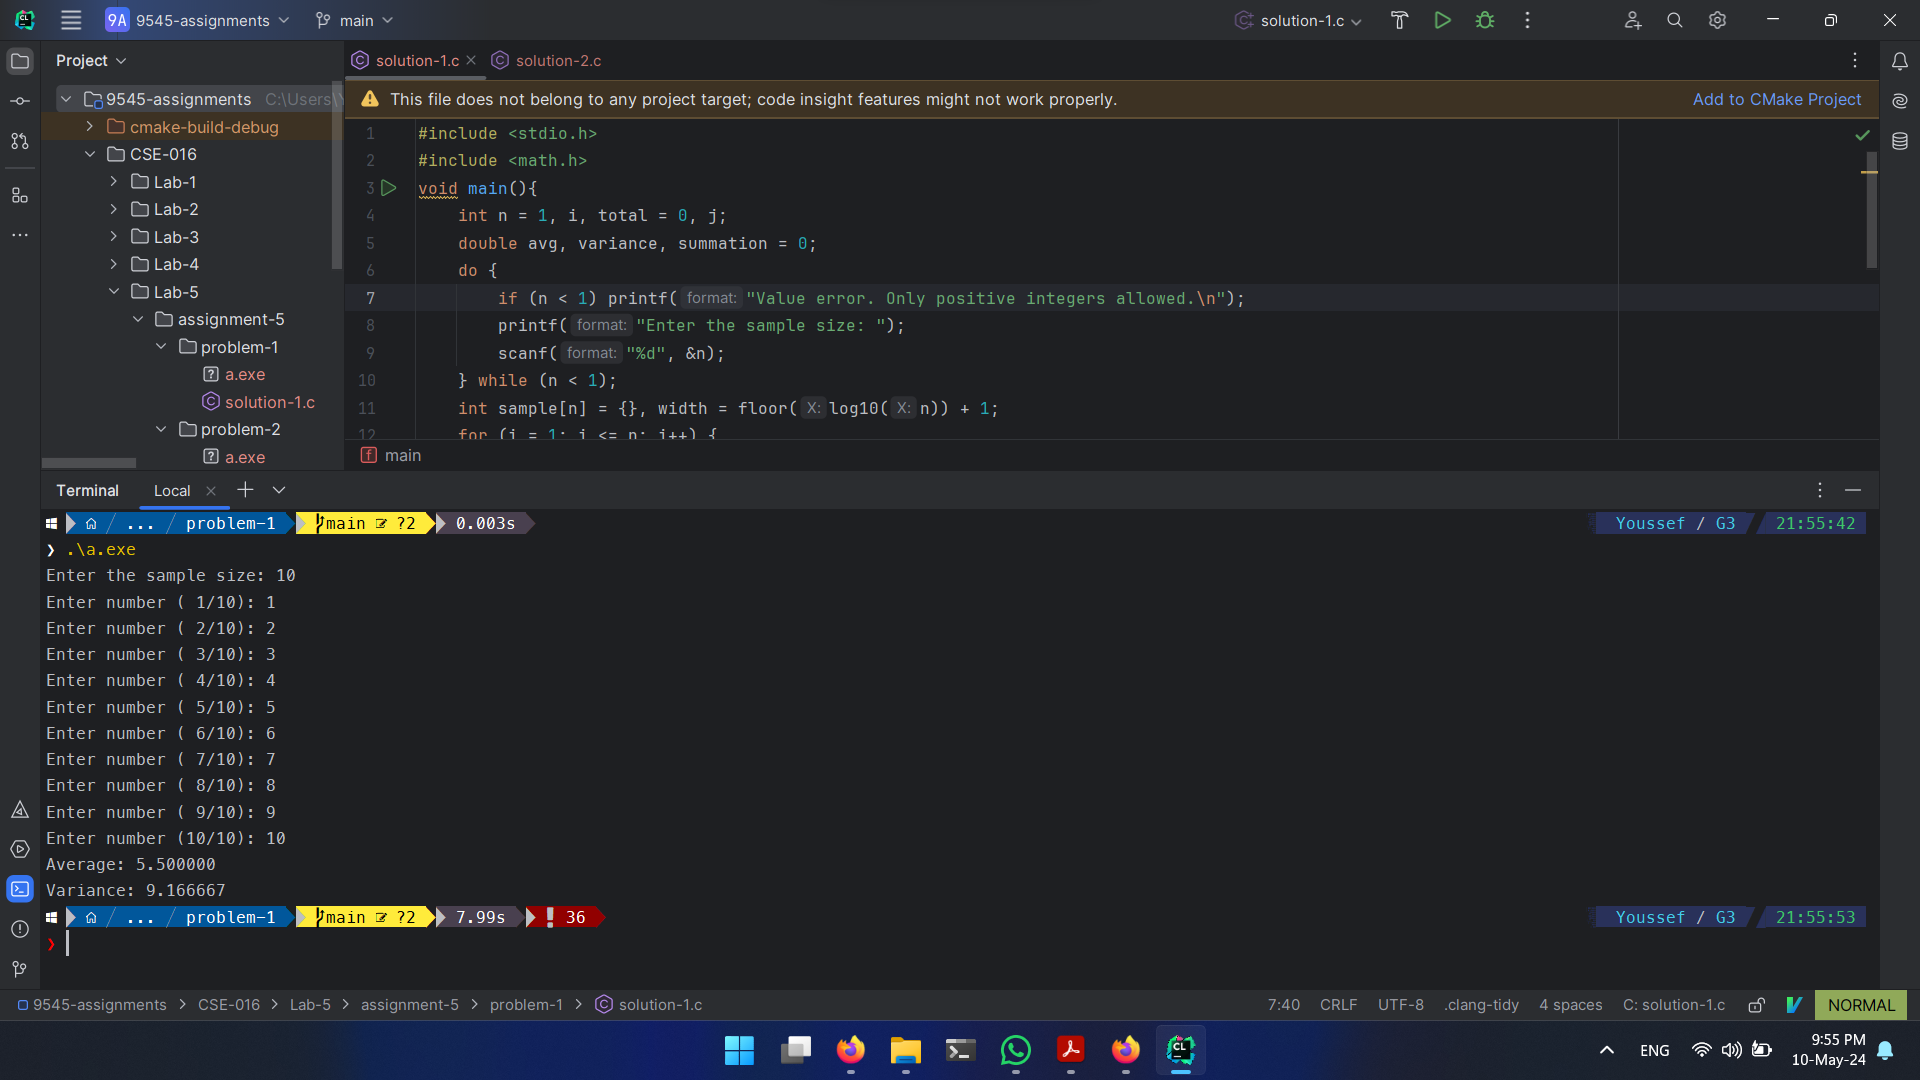
\includegraphics[width=\linewidth]{assets/prob-1.png}
    \caption{Desktop screenshot of Problem (1)'s code in CLion}
\end{figure}
\begin{figure}[!h]
    \centering
    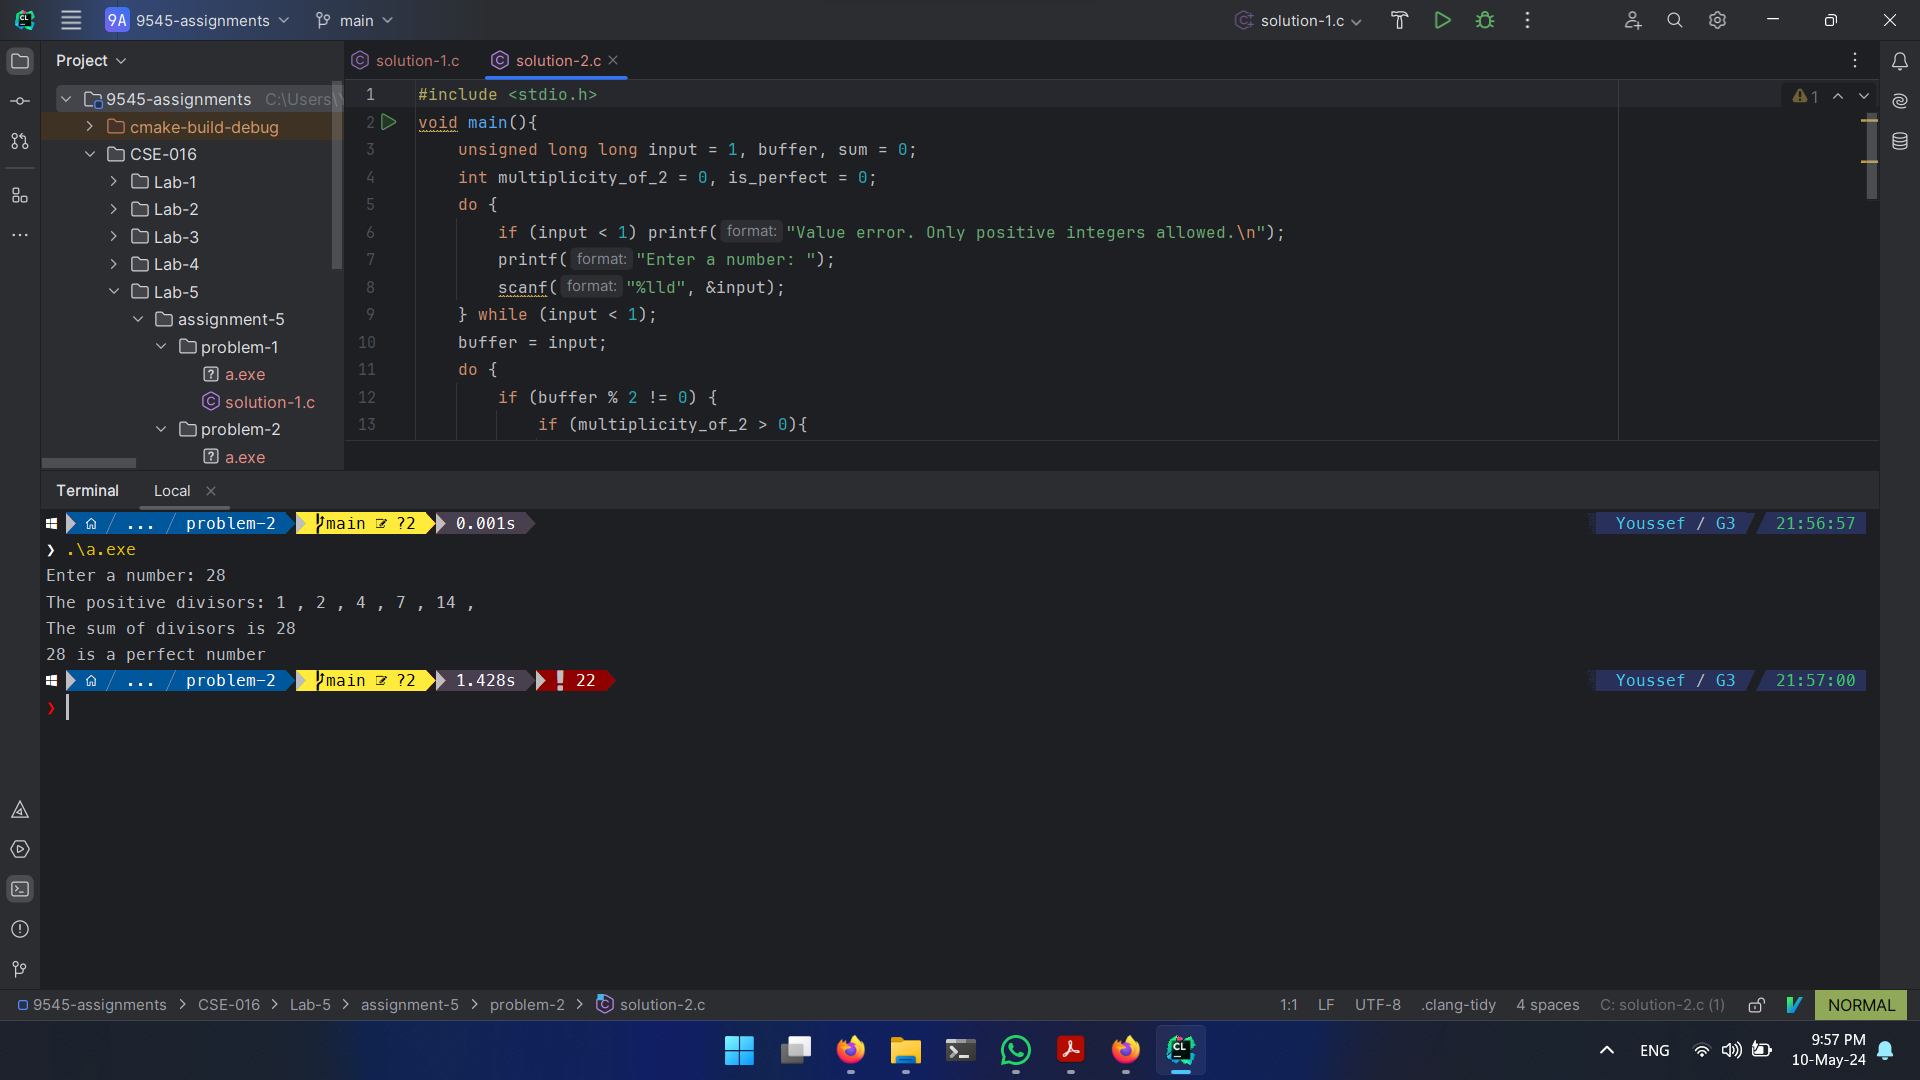
\includegraphics[width=\linewidth]{assets/prob-2.png}
    \caption{Desktop screenshot of Problem (2)'s code in CLion}
\end{figure}
\newpage
\subsection{Specifications}
\begin{itemize}
    \item \textbf{Libraries:}
    \begin{itemize}
        \item \texttt{\color{inlinecode}{stdio.h}}
        \item \texttt{\color{inlinecode}{math.h}} (problem 1)
    \end{itemize}
    \item \textbf{Compiler:} GNU C Compiler \texttt{\color{inlinecode}{(gcc)}} version 13.2.0 (x86\_64-posix-seh-rev1)
    \item \textbf{C Standard Compatibility}
    \begin{center}
        \begin{tabular}{|c|c|c|c|c|c|}
             \hline
             \textbf{P\#} & \textbf{C89/C90} & \textbf{C99} & \textbf{C11} & \textbf{C17} & \textbf{C23} \\
             \hline
              1 & \checkmark & \checkmark & \checkmark & \checkmark & \checkmark \\
              2 & \checkmark & \checkmark & \checkmark & \checkmark & \checkmark \\
             \hline
        \end{tabular}
    \end{center}
    
    %\begin{flushright}
    %    \begin{tabular}{c|c}
    %         Symbol & Compatibility  \\
    %         \hline
    %         \checkmark & Full \\
    %         $\sim$ & Non-Fatal Errors \\
    %         $\times$ & Incompatible
    %    \end{tabular}
    %\end{flushright}
    \item \textbf{Supported Platforms:} OS: (any), architecture: (any)
    \item \textbf{Tested On:} Windows 11 64-bit
\end{itemize}
\section{Licenses}
This document, my additions to its \LaTeX \ source code, the software included and its \texttt{C} source code all come without warranty and are all subject to the BSD 3-Clause Open Source License:\\https://opensource.org/license/bsd-3-clause.\\

\begin{center}
    COPYRIGHT \copyright \ 2024, Youssef Ahmed Samy
\end{center}
\fancypagestyle{lastpage}
{
   \fancyhf{}
   \fancyfoot[C]{\textsl{END OF DOCUMENT}}
   \fancyfoot[L]{Assignment 5}
    \rfoot{Page \thepage \ of \pageref{LastPage}}
}
\thispagestyle{lastpage}
\end{document}
